\documentclass[12pt]{article}

\usepackage{sbc-template}
\usepackage{graphicx}

% http://tex.stackexchange.com/questions/45498/choosing-whether-to-include-pdf-or-png-in-pdflatex
\DeclareGraphicsExtensions{%
    .pdf,.PDF,%
    .png,.PNG,%
    .jpg,.mps,.jpeg,.jbig2,.jb2,.JPG,.JPEG,.JBIG2,.JB2}

\usepackage[hyphens]{url}
%\usepackage[brazil]{babel}
\usepackage[utf8]{inputenc}
\usepackage{hyperref}

\sloppy

\title{Patterns for Engagement in Free Software Projects}
\author{Antonio Terceiro\inst{1}, Rodrigo Souza\inst{2}, Christina Chavez\inst{3}}

\address{Cooperativa de Tecnologias Livres (Colivre)\\
Salvador, BA -- Brazil\\
terceiro@dcc.ufba.br
\nextinstitute
Superintendência de Tecnologia da Informação (STI)\\
Federal University of Bahia (UFBA)\\
Salvador, BA -- Brazil \\
rodrigo@dcc.ufba.br
\nextinstitute
Departamento de Ciência da Computação (DCC)\\
Federal University of Bahia (UFBA)\\
Salvador, BA -- Brazil\\
flach@dcc.ufba.br
}

\begin{document}
\maketitle

\begin{abstract}
Free/Libre/Open Source Software (FLOSS) projects are developed in a collaborative manner, 
by communities of contributors that work on publicly available source code.
However, many potential contributors are still daunted by the FLOSS world.
The \textit{Patterns for Engagement in Free Software Projects} 
present solutions for recurring problems that emerge when
prospective contributors are willing to select a FLOSS project
to get involved and to contribute with.
They are organized around three clusters: 
(a) \textit{Selection Patterns}, that help prospective contributors to find suitable projects, 
(b) \textit{Involvement Patterns}, that deal with the first steps towards 
getting familiar and involved with the selected project, and 
(c) \textit{Contribution Patterns}, that document best practices for submitting 
different kinds of contribution to a free software project. 
The \textit{Patterns for Engagement in Free Software Projects} catalog is itself a FLOSS project. 
Its license allows free reuse of the text, as long as the modified versions 
are distributed under the same license.
\end{abstract}

%-------------------------------------------------------------
\section{Introduction}

Free/Libre/Open Source Software (FLOSS) is a class of software projects
that have Internet-based interaction between developers and public
source code licensed under terms that comply with either the Free
Software definition by the Free Software Foundation
(FSF)\footnote{http://www.gnu.org/philosophy/free-sw.html} or the Open
Source Definition by the Open Source Initiative
(OSI)\footnote{http://www.opensource.org/docs/definition.html}.

A FLOSS project starts when an individual developer, or an organization,
decides to make a software product publicly available on the Internet so that
it can be freely used, modified, and redistributed \cite{kon2011}.
After an initial version of a FLOSS project is released and advertised in 
the appropriate communication channels, it may be subject to 
different kinds of contributions 
-- for instance, development of new features, bug fixing, testing, documentation --
performed by a plethora of contributors, 
in which standard techniques and practices are often used.
However, many potential contributors are daunted by 
what they imagine is a high barrier to entry into the FLOSS world \cite{lester2012}.
%Indeed, there may be some barriers to overcome, possible as high as those ones you have to deal with when  moving to a new school or getting a new job.

\textit{Patterns for Engagement in Free Software Projects} 
-- or \textit{Free Software Patterns},  for short -- 
present solutions for recurring problems that emerge when
prospective contributors are willing to select  an open source software project
to get involved and to contribute with.
 \textit{Free Software Patterns} describe alternative ways of
selecting and getting familiar with FLOSS projects,  
and entail activities that go beyond programming or reporting bugs,
such as documenting, performing translations and writing tests.

\textit{Free Software Patterns} are organized around three clusters of patterns.  
Figure~\ref{fig:clusters} shows the clusters and their relationships. 
Each cluster is presented as a simple pattern language, conceived to
document and to address a common set of problems that 
prospective contributors to FLOSS projects face:
%The three clusters of patterns are:
\begin{itemize}
  \item
    \emph{\textit{Selection Patterns}} help prospective contributors to 
    find and select suitable FLOSS projects to contribute with.
  \item
    \emph{\textit{Involvement Patterns}} help prospective contributors to 
    get familiar with FLOSS projects and figure out where to start.
  \item
    \emph{\textit{Contribution Patterns}} help prospective contributors to
    actually perform contributions to FLOSS projects. These patterns
    are organized according to the type of contribution,
    that is, documenting, translating, reporting bugs, resolving bugs,
    adding features, and so on.
\end{itemize}

\begin{figure}[hbt]
  \begin{center}
    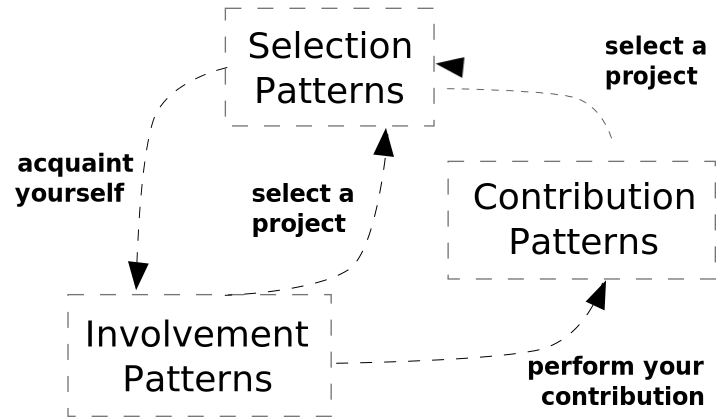
\includegraphics[width=0.6\textwidth]{figures/clusters}
  \end{center}
  \caption{Free Software Patterns Overview}
  \label{fig:clusters}
\end{figure}

Patterns are particularly well-suited for presenting and discussing
techniques and practices. 
For instance, the Reengineering Patterns~\cite{demeyer2008}  present solutions 
for  recurring software reengineering problems. 
Each pattern describes one part of
the reengineering process and produces different kinds of outputs, such as 
refactored code or insights into how the system functions~\cite{demeyer2008}.
\textit{Selection Patterns} and \textit{Contribution Patterns} are
intrinsically associated with the nature of FLOSS projects, 
and represent original work. 
\textit{Involvement Patterns} include two new patterns documented by us,
but also reuse some  Reengineering Patterns,
for instance, the \textit{ First Contact} patterns ~\cite[p.~39]{demeyer2008},
that help developers when they encounter a legacy system
(not necessarily FLOSS) for the first time.

%-----------------------------------------------------------------

The presentation of \textit{Selection Patterns} (Section~\ref{sec:selection}) and
\textit{Involvement Patterns} (Section~\ref{sec:involvement})
follows the approach to pattern description used in the 
Object-Oriented Reengineering Patterns (OORP) book~\cite{demeyer2008}.
The description of a cluster includes an overview, 
the forces that influence its set of patterns,
and a map of these patterns, depicting how they may be related.  
For each pattern in the cluster, the following fields for pattern documentation
are presented: 
pattern name, intent, motivation, problem, forces, solution, trade-offs, rationale,
known uses, related patterns and next steps. 
The cluster description ends up with closing remarks and a brief discussion
about its set of patterns. 

\textit{Contribution Patterns} (Section~\ref {sec:contribution}), however,
are still work in progress and, therefore, they are presented 
as short descriptions of their proto-patterns, 
also known as \textit{patlets}.

%-----------------------------------------------------------------
\section{\textit{Selection Patterns}} \label{sec:selection}

%You want to contribute to a FLOSS project for several different reasons.
You have either been building systems with existing FLOSS projects or 
have been involved with using FLOSS, or 
have an interest for contributing to some existing FLOSS projects.
%
You can have extrinsic motivations for contributing, 
such as improvement of programming skills, 
creation of required and unavailable code, 
and enhancement of professional status,
or intrinsic motivations, such as altruism, fun, reciprocity, 
intellectual stimulations, and a sense of obligation to contribute~\cite[p.~2058]{oreg2008}.

When selecting a project, it is often the case that 
there are several repositories that list FLOSS projects, for instance, 
SourceForge\footnote{\url{http://sourceforge.net/}} and Ohloh\footnote{\url{http://www.ohloh.net/}}.
You navigate through some projects in these repositories but still have no
clue about which FLOSS project could be a good starting point.
You feel somewhat lost and concerned: there are several interesting projects, 
that use different technologies and programming languages, possibly with different 
development processes and types of participation. 
Is  there a strategy for selecting a FLOSS project, 
that takes into account your motivations to contribute?
%Question:	
How do you select a FLOSS project to contribute, 
aligned with your motivation?   % and be encouraged to keep on contributing?

\subsection{Global Forces}

The patterns in this cluster must resolve the following forces:
\begin{itemize}

\item \textit{Basic Needs.} 
You need software to get your work done, and you do not have the
resources to create them from scratch. Therefore, you have to find existing
software that implements at least a large subset of the features you need.

\item \textit{Familiarity.} 
Previous use of a FLOSS project tends to facilitate your work and increase your motivation to contribute.
You may be aware of existing features, bugs and enhancements that are necessary. 
This may ease your work as contributor.

\item \textit{Expertize on some technology.}
You will possibly provide better contributions for projects that use
languages and technologies that you happen to master.

\item \textit{Reputation issues.}
Contributing to a FLOSS project implies in social interaction with other contributors 
in a new environment, and reputation-related issues and concerns may naturally arise.
Reputation is gained by convincing your peers that you know what 
you are doing or talking about. 
This can be wonderful for you self-esteem and may also bring good jobs.

%“Start by doing what's necessary; then do what's possible; and suddenly you are doing the impossible.” St. Francis of Assisi 
\item \textit{Feasibility.} It is self-rewarding to select a task, 
and spend some effort on it through its completion.
You want to select a project in which performing contributions is 
feasible, that is,  you will be able to successfully contribute 
and will be motivated to keep on contributing.
Changeability, i.e. the ease of accommodating future changes, 
can be a major dimension on the feasibility of your contribution.

\item\textit{Don't reinvent the wheel}. Think about a functionality. 
Probably, it has already been implemented
by one or more open source software projects. 
Common wisdom recommends that you invest some time on searching
for existing software that implements the desired features, 
before trying to develop a new software from scratch.
Developing a software from scratch is not simple and requires time.

\end{itemize}

\subsection{Overview}

Selection Patterns help prospective contributors to find suitable FLOSS projects to contribute with, 
depending on some criteria. 
Figure~\ref{fig:selection} presents the three patterns that comprise this cluster.

\begin{figure}[hbt]
  \begin{center}
    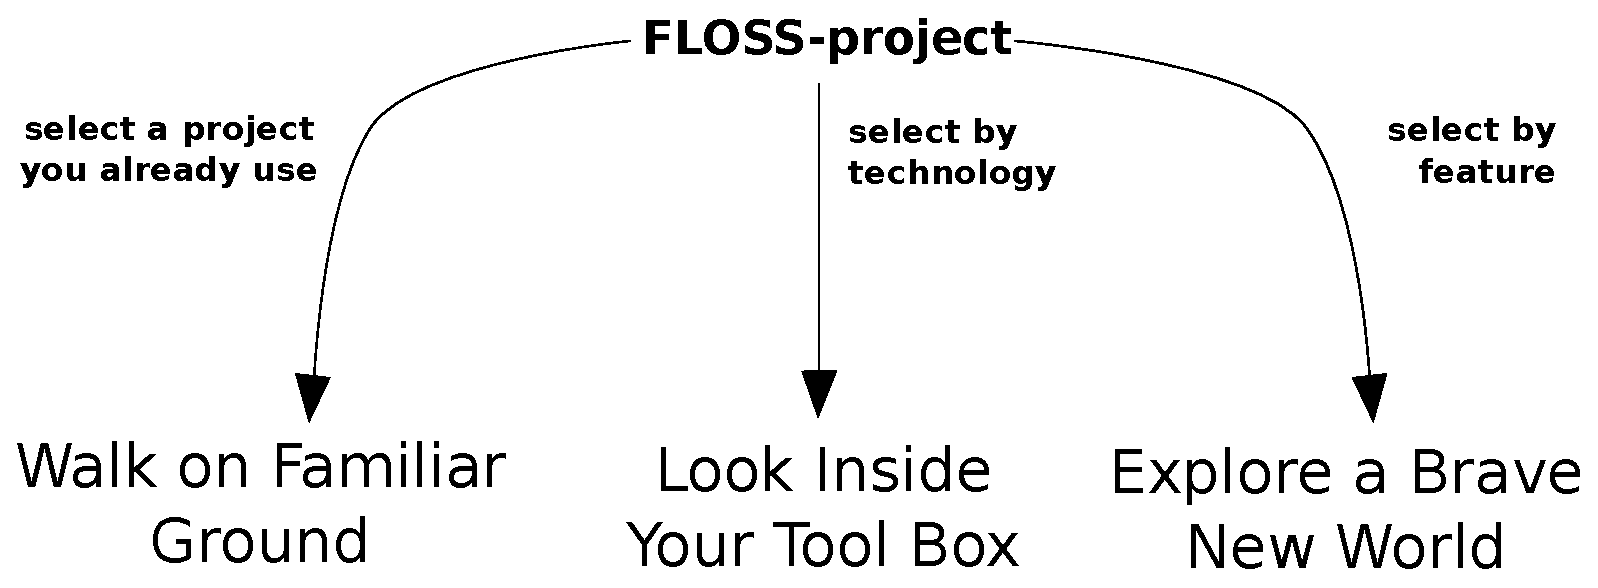
\includegraphics[width=\textwidth]{figures/selection}
  \end{center}
  \caption{Selection Patterns}
  \label{fig:selection}
\end{figure}

%Explaining Figure 1 - Pattern overview. TO BE IMPROVED
You should 
\textit{Walk on Familiar Ground} (Section~\ref{selection/WalkOnFamiliarGround})
to select  an open source project that you already use and are somewhat familiar with.
Or maybe you prefer to
\textit{Look Inside your Toolbox} (Section~\ref{selection/LookInsideYourToolBox})
and select a project based on the technologies that  you know and feel somewhat confident to use.  
Yet another possible path is to 
\textit{Explore a Brave New World} (Section~\ref{selection/ExploreABraveNewWorld}) 
whenever you are willing to select a project based on the features or functionalities 
it provides, despite the risk of having to deal with unknown technologies. 

\input{../selection/WalkOnFamiliarGround.ltx}
\input{../selection/LookInsideYourToolBox.ltx}
\input{../selection/ExploreABraveNewWorld.ltx}

\subsection{Discussion}

\textit{Selection Patterns}, although presented separately for clarity, 
can be used together in different situations.
For example, while considering to \textit{Walk On Familiar Ground}
(Section~\ref{selection/WalkOnFamiliarGround}) 
you may select a project that uses unfamiliar technologies, 
and in this case, you should also consider  forces and
trade-offs as if you were about to \emph{Explore a Brave New World}
(Section~\ref{selection/ExploreABraveNewWorld}).

Functionality can be used as an alternative criteria for selecting a project to
contribute with. If you are considering to
\textit{Look Inside your Tool Box} (Section~\ref{selection/LookInsideYourToolBox}),
functionality may help you to choose among alternative projects 
that use the same underlying acceptable technologies.

If a team is willing to select a FLOSS project, 
the use of \textit{Selection Patterns} may not be straightforward.  
For instance, when you 
\textit{Look Inside your Tool Box} (Section~\ref{selection/LookInsideYourToolBox})
to select a project, some of the team members may already know the technology, 
while other members may still have to learn it.
Likewise, the selected project may be familiar to and used by some
but not all team members.

Finally, the use of \textit{Involvement Patterns} (Section~\ref{sec:involvement})
can expose difficulties and risks related to some selected FLOSS project that may
result in yet  another round of using \textit{Selection Patterns}.

%--------------------------------------------------------------
\section{\textit{Involvement Patterns}} \label{sec:involvement}

You have selected an open source project to contribute with, 
maybe one that you already use or that implements features you need. 
But it is possibly a large project, with several thousands of lines of code, 
dozens of developers, bug tracking systems with lots of bugs to be fixed, and so on. 
Moreover, FLOSS projects are mostly developed in a public, 
collaborative manner, by a community of contributors.
These FLOSS communities often determine the way things are done in the project.
You want to contribute with the selected project but first you need to get familiar 
with the software and get involved with the project ecosystem -- that 
includes its community and the way things are done.

Are there any strategies to becoming familiar to 
a FLOSS project that should be considered?
How can you get involved with a FLOSS project in a short amount of time, 
so that you can start to contribute as early as possible?

% pdf p. 58
\subsection{Global Forces}
\begin{itemize}
\item \emph{Software systems are often large and complex}. In such cases, it is
not practical to try to understand the whole system before you start contributing.

\item \emph{Software evolves}. Even if you manage to fully  understand the 
system, by the time you finish, the system would probably be different from 
that one you studied. 

\item \emph{You are an outsider}. Chances are that nobody knows you in the
project community. Current developers may not trust you with 
important contributions until you show your abilities while contributing with small changes. 
Or maybe you need to build self-confidence before making contributions with a higher
level of difficulty.

\item \emph{Contributions are welcome}. Usually, even small contributions are
well received by free software projects, especially when they address issues
recognized as important by the community.

\end{itemize}

%Explaining Figure 2 - Pattern overview. TO BE IMPROVED
\subsection{Overview}

Involvement Patterns deal with the first steps towards getting familiar with the selected 
FLOSS project and involved with its environment.
Figure~\ref{fig:involvement} presents the patterns that comprise this cluster.
\begin{figure}[hbt]
  \begin{center}
    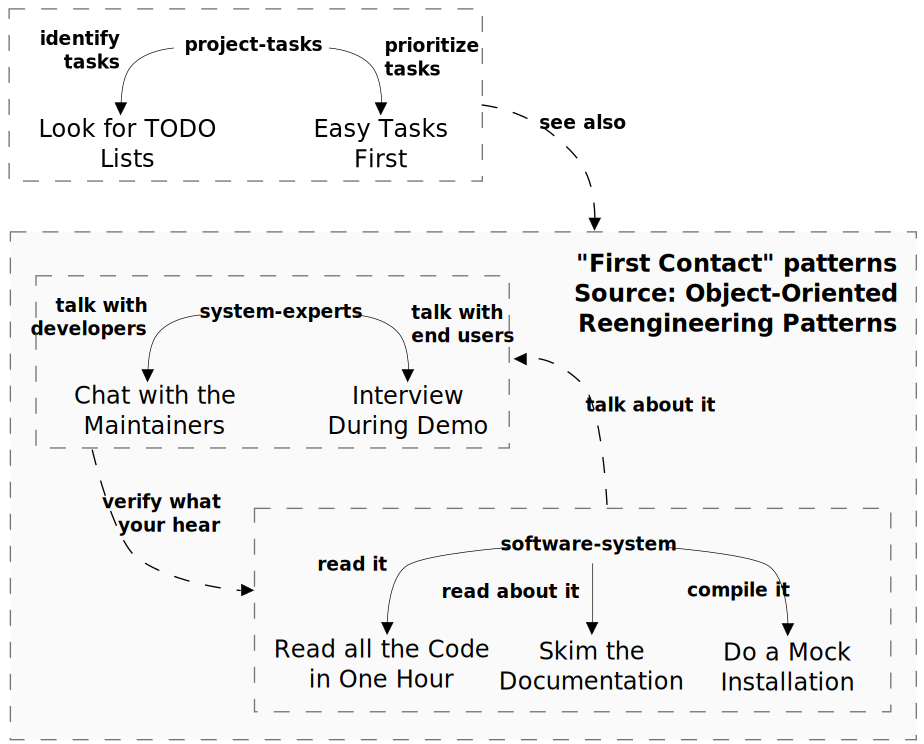
\includegraphics[width=\textwidth]{figures/involvement}
  \end{center}
  \caption{\textit{Involvement Patterns}}
  \label{fig:involvement}
\end{figure}

\textit{First Contact} \cite{demeyer2008} consists of a set of patterns for reverse engineering 
that may be useful when you encounter a legacy system for the first time.  
FLOSS projects are legacy systems, and therefore  these patterns may  be useful for helping 
you to get familiar with a FLOSS system that is completely new for you. 
The intents of the patterns that comprise the \textit{First Contact} cluster 
are listed in the Appendix~\ref{sec:appendix}.

\textit{Look for Todo Lists} (Section~\ref{involvement/LookForTodoLists}) and 
\textit{Easy Tasks First} (Section~\ref{involvement/EasyTasksFirst}) are
patterns that can be useful when you are already getting familiar with the FLOSS 
software but still not sure about where and how you should start to contribute.
Both patterns can help you to get acquainted with the community and 
the way things are done in the FLOSS project.

\input{../involvement/LookForTodoLists.ltx}
\input{../involvement/EasyTasksFirst.ltx}

\subsection{Discussion}

\textit{Involvement Patterns} describe strategies that can be used to walk the
first steps in contributing to a project. 
The \textit{First Contact} patterns~\cite{demeyer2008} help
prospective contributors in getting acquainted with the FLOSS product.
The other two complementary patterns --
\textit{Look for Todo Lists} and \textit{Easy Tasks First} 
--  help them in getting partially familiar with the FLOSS process.
However, the applicability of these patterns
relies on specific resources that may or may not be found within a project,
for instance, TODO annotations in source code and lists of easy tasks. 

It is often a good idea to apply the \textit{First Contact} patterns \cite{demeyer2008}
to get familiar with  FLOSS projects that are new for you
or your team in a short amount of time.
%
The patterns  \textit{Chat with the Maintainers} ((Section~\ref{involvement/ChatWithMaintainers}) 
and \textit{Interview During Demo} ((Section~\ref{involvement/InterviewDuringDemo})  
help you get acquainted with the people involved in conventional projects 
in the context of software reengineering \cite{demeyer2008}.
However,  while \textit{Chat with the Maintainers} can be adapted for the FLOSS setting
(for instance, by using IRC channels),
\textit{Interview During Demo} 
will not be of much help to get you  acquainted with contributors and the FLOSS itself.

Finally, the use of \textit{Involvement Patterns} can expose problems and risks 
related to the selected FLOSS project that may
result in yet  another round of using \textit{Selection Patterns} (Section~\ref{sec:selection})
to choose alternative projects for which contributions are feasible.

%---------------------------
\section{\textit{Contribution Patterns}} \label{sec:contribution}

Your desire to contribute to a FLOSS project is well underway. 
You selected a project, you became familiar with the legacy free software and 
you even identified possible starting points for contributing.
How can you be sure that you will provide useful contributions, 
and that they will be accepted by project leaders? 
And what about your reputation if your contributions provide some undesirable effects to the project?
Can you start with tasks other than coding or fixing bugs?

\subsection{Forces}
\begin{itemize}
\item \textit{Fear of rejection.} You are concerned about possible barriers to entry into a FLOSS project or to have your contributions rejected by project leaders.
\item \textit{Lack of Confidence.} You lack confidence on your programming or other technical skills; 
this may be an hindrance on your ability to  make ``good'' contributions.
\item \textit{Lack of Time.} Your available time may not be enough to allow you to make relevant contributions.
\end{itemize}

\subsection{Overview}

\textit{Contribution Patterns} document best practices for submitting different
kinds of contribution to a FLOSS project, such as, reporting bugs, discussing problems, writing documentation, 
performing translations, fixing bugs, creating tests, developing features, among others.

At the moment, the \textit{Contribution Patterns} are work in progress.
Therefore, in this section, we present them only as proto-patterns, with a name and intent. 
We are currently working on expanding and  writing down these patterns in more detail 
and we plan to make them available in future publications.
Figure~\ref{fig:contribution} presents the patlets in this cluster.

\begin{figure}[hbt]
  \begin{center}
    \includegraphics[width=\textwidth]{figures/contribution}
  \end{center}
  \caption{Contribution Patterns}
  \label{fig:contribution}
\end{figure}


\subsubsection{Write Documentation} \label{contribution/WriteDocumentation}
    Contribute to a free software project by writing useful documentation.
\subsubsection{Translate To Your Language} \label{contribution/TranslateToYourLanguage}
     Contribute to a free software project by translating documents and software to your language.
\subsubsection{Review Recent Activity} \label{contribution/ReviewRecentActivity}
    Identify news and opportunities related to the software project.
\subsubsection{Right Version for the Task} \label{contribution/RightVersionForTheTask} 
    Bug fixes in stable versions, new features in the development version.
\subsubsection{Create a Patch} \label{contribution/CreatePatch}
    Produce a file that fully describes your changes to the source code of the project.
\subsubsection{Add Failing Tests} \label{contribution/AddTestsThatFail} 
    Reproduce bugs in a automated way so that they don't come bac   later.
\subsubsection{Review Your Changes}  \label{contribution/ReviewYourChanges}
    Put yourself in the project leaders' shoes, and review your own work.
\subsubsection{Explanatory Commit Messages} \label{contribution/ExplanatoryCommitMessages}
    Make it easier for other people to understand the reasons for a change.
\subsubsection{Document Your Changes} \label{contribution/DocumentYourChanges} 
    Update relevant documentation when adding new features or modifying existing ones.
\subsubsection{Group Related Changes} \label{contribution/GroupRelatedChanges} 
    Submit related changes as a single patch.
\subsubsection{Separate Unrelated Changes} \label{contribution/SeparateUnrelatedChanges} 
    Submit unrelated changes in separate patches to ease the review.
\subsubsection{Manual Testing} \label{contribution/ManualTesting}
    Test features by manually executing the software.
\subsubsection{Write Useful Bug Reports} \label{contribution/WriteUsefulBugReports}
    Provide all the information needed for other people to reproduce the bug you found.
   

\section{Conclusions}

In this paper, we presented the \textit{Free Software Patterns}, which are organized
around three clusters: \textit{Selection Patterns}, \textit{Involvement Patterns}, and
\textit{Contribution Patterns}.

These clusters are meant to guide potential contributors
from project selection to involvement, and then to actual contributions. 
There is a strong interplay between Selection Patterns and Involvement Patterns: it
is often necessary to get involved with a project in order to gather relevant
information --- e.g., quality of the documentation --- before deciding if it is
worth contributing to or if it is better to select another project.

Although free software projects tend to be open to participation, it is not
always easy to find a suitable project and get involved in the community~\cite{lester2012}. 
This set of patterns should help potential contributors by documenting in a
structured format some useful advices and best practices from free software
communities. 

% TODO: the FSP should suit various situations: people who want to translate,
% document, to use and extend software in a corporation, hobbysts who want to
% learn a new programming language, users who want to improve the software they
% use and get involved in the community...

We have briefly described an outline of the \textit{Contribution Patterns}. 
We are currently working on expanding and  writing down these patterns in more detail.
As future work, we intend to refine the  \textit{Free Software Patterns} with the
experience gained from applying them in an
practical course on free software development.

The \textit{Free Software Patterns} catalog is itself an open project. Its
license allows free reuse of the text, as long as modified versions are made
available under the same license. Anyone interested in sharing experiences and
points of view is welcome to contribute with new patterns and refinements by
visiting the official pattern repository\footnote{Source available at\\
\url{https://gitorious.org/flosspapers/free-software-patterns/}.}.

\appendix

\section{\textit{First Contact}, from Object-Oriented Reengineering Patterns \cite{demeyer2008}} \label{sec:appendix}

\subsection{\textbf{Chat with the Maintainers}} \label{involvement/ChatWithMaintainers}
    Learn about the historical and political context of your project
    through discussions with the people maintaining the system.
    
\subsection{\textbf{Do a Mock Installation}} \label{involvement/DoAMockInstallation}
    Check whether you have the necessary artefacts available by
    installing the system and recompiling the code.

 \subsection{\textbf{Interview During Demo}} \label{involvement/InterviewDuringDemo}
    Obtain an initial feeling for the appreciated functionality of a
    software system by seeing a demo and interviewing the person giving
    the demo.
    
\subsection{\textbf{Read the Code in One Hour}} \label{involvement/ReadTheCodeInOneHour}
    Assess the state of a software system by means of a brief, but
    intensive code review.
    
\subsection{\textbf{Skim the Documentation}} \label{involvement/SkimTheDocumentation}
    Assess the relevance of the documentation by reading it in a limited
    amount of time.


\section*{Acknowledgements.}
A very special ``thank you'' for  Joe Yoder, for his invaluable availability, dedication and effort in shepherding us.
We are also grateful to Serge Demeyer, St\'{e}phane Ducasse and Oscar Nierstrasz for having licensed the
Reengineering Patterns under the Creative Commons Attribution-ShareAlike 3.0 Unported license,
which allowed us to partially base our own work on theirs. 
Last but not least, we would like to thank -- 
for their supportive interaction and  rich discussions during our lectures and meetings in 2012 -- 
Mario Jorge Pereira, Rafael Glauber Silva, Sergio Gramacho, Luciana Silva, 
Debora Nascimento, Thiago Colares, Thiago Mendes, Vagner Amaral, 
Aline Meira, Patricia Melo, Murilo Botelho, Alvaro Lordelo and Tiago Motta.

\bibliographystyle{sbc}
\bibliography{fsp2012}

\end{document}
